%======================================================================
%===  dtuposter - a class to make posters tha comply with the DTU CI
%
% Written and maintained in 2011-2014 
% by Jorrit Wronski (jowr@mek.dtu.dk)
%
%
%==========================================
%===  details and poster setup
\documentclass[
    ,title     = {{Methods for image classification}}
    ,longtitle
%    ,author    = {{Anders Launer Bæk}}
%    ,subject   = {{This is the subject of my work}}
%    ,bgcolor   = dtulightgreen
    ,highlight = dtured
    ,toplogo   = {{template/tex_dtu_compute_b_uk}}
    ,botlogo   = {{template/tex_dtu_frise}}
    ,papersize = {{a0paper}}
    ,colcount  = {{3columns}}
%    ,largecaption
%    ,draft
%    ,nocrop
%    ,fleqn          % equations on the left
]{dtuposter}
%======================================================================
%=== Font definitions, DTU recommends Arial for posters
\usepackage{cmbright}
\usepackage{arevmath}
\usepackage{pgfplots}
\usepackage{wrapfig}
\usepackage{graphicx}
\usepackage{subcaption}
\usepackage{tikz}
\renewcommand{\familydefault}{\sfdefault}
\usepackage[bottom]{footmisc}
\usepackage{enumitem}
\usepackage{multirow}
\usepackage{lipsum}
\setlist{nosep,leftmargin=*}
%======================================================================
%=== Other useful packages
\usepackage[utf8]{inputenc}
\usepackage{booktabs}
\usepackage{siunitx}
\usepackage{todonotes}
\graphicspath{{./Figures/}}
%======================================================================
%=== The actual content starts here
\begin{document}
%===  Make header for poster (title and authors)
\begin{dtuposterhead} %
\dtuposterauthor{Tim F. Olsen, Marcus K. Nielsen \& Anders L. Bæk.}
\dtuposteraffil{Case 2 in 02582 Computational Data Analysis}
\end{dtuposterhead}
%
%
%======================================================================
%===  ... and the rest of the content
\begin{minipage}{\textwidth}
%======================================================================
%===  Introduction part
\section*{Introduction}

\begin{wrapfigure}{r}{0.33\textwidth}
\centering
\vspace{-12cm}
\begin{subfigure}[t]{0.15\textwidth}
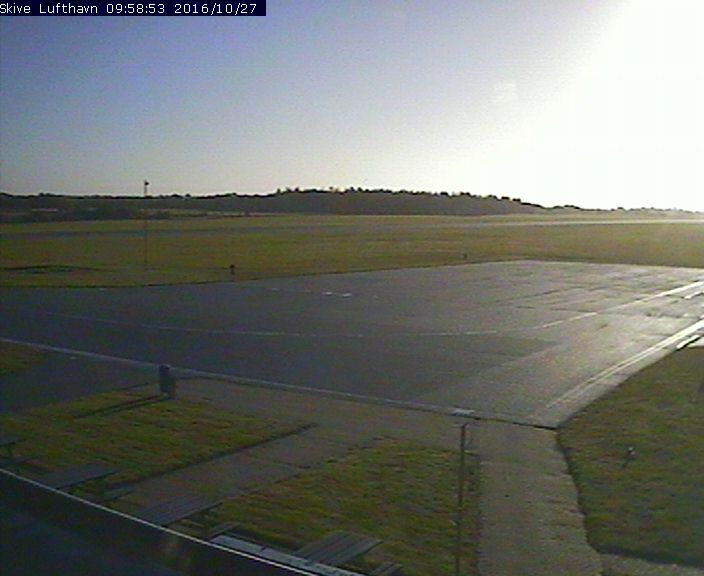
\includegraphics[width=\textwidth]{clear_example}
\end{subfigure}
\begin{subfigure}[t]{0.15\textwidth}
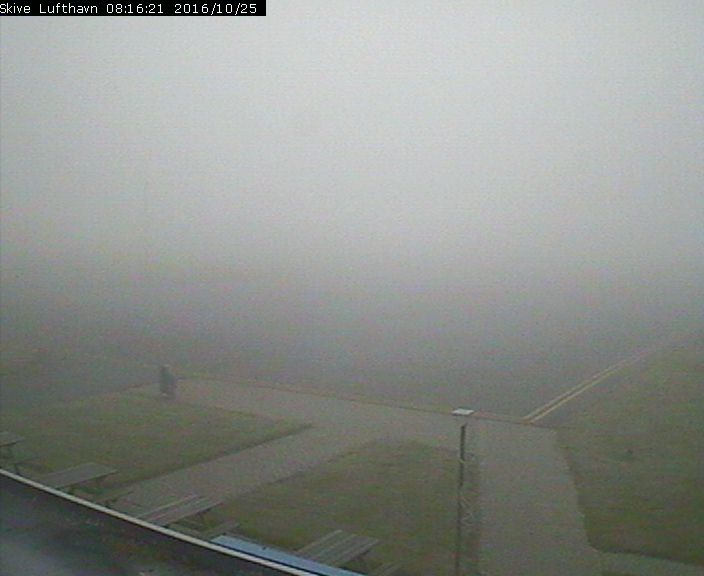
\includegraphics[width=\textwidth]{foggy_example}
\end{subfigure}
\caption{Examples of the data we are working on. The left image is classified as clear and the right is classified as foggy.}
\vspace{-1cm}
\end{wrapfigure}

DMI have asked the participants of this course to attempt to classify a number of images of foggy and clear roads and scenes. Our take on the problem is to test two different methods for classifying the images: A manual extraction of features and a convolutions deep artificial neural network (ANN).

The data sets we have available contains both clear and foggy images, but it is very skewed with about 1.500 foggy images and 150.000 clear images. Additionally there exists duplicates and the images are not independent since they are taken within a short time frame.


%\subsection{limitations}


%\todo[inline]{Der er ikke foretaget nogen kritik af allerede lablet billeder..}

%\todo[inline]{Fælles for begge: overvejelser omkring IID og gentagende billeder.}

%\todo[inline]{Jeg kan ikke få den til at vise footnotes? hvertfald ikke det rigtige sted.}

%===  End of Introduction part
%======================================================================

\vspace{1cm}
\hrule
\vspace{1cm}
\end{minipage}
\begin{minipage}[t]{0.30\textwidth}
%======================================================================
%===  Anders' part
\section*{Feature extraction approach}

The main goal of the hand crafted feature extractions is to see how well they are to generalize across locations.
The model has been trained on images from Skive and the test of generalization are measured on a subset of the Billund images.
\paragraph{Features:} The extracted features were; the mean value of the Dark channel, the variance and the squared sum of the Sobel filter values, the absolute sum and variance of the Laplace filter and the pct. of overexposed pixels\footnotemark[1]. 
All features have been adjusted to the size of the image to create a standard of reference.

Figure \ref{fig_rfc_1} illustrates the properties of the features by the first and second PCA.% principal components. %The features are clustering and separating the clear weather images and the fog images nicely.

\begin{figure}
\centering
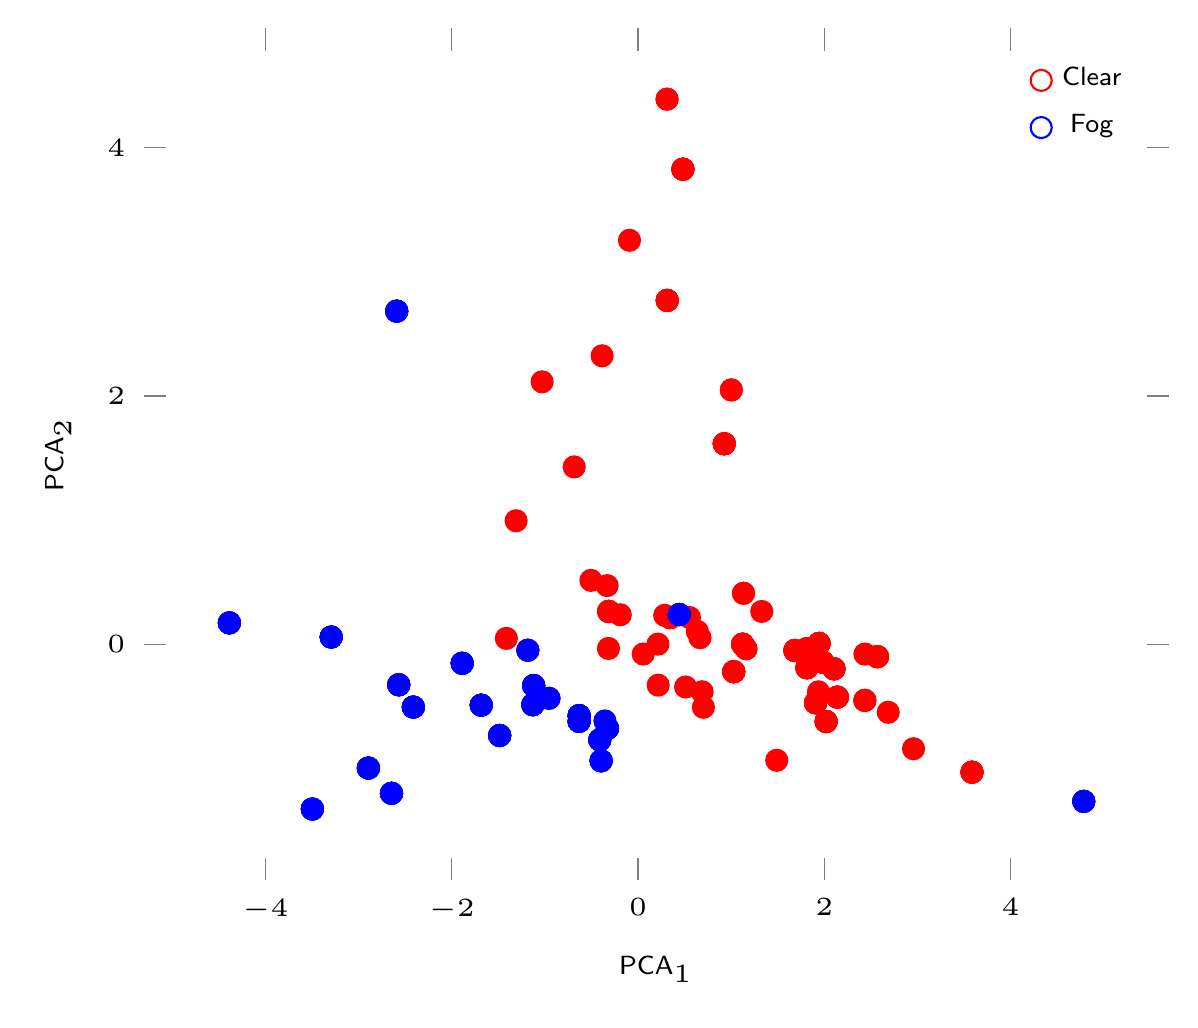
\begin{tikzpicture}[scale=1.9]
\begin{axis}[axis line style={draw=none},
legend style={fill=none, fill opacity=0, draw=none, draw opacity=1, text opacity=1},
    xlabel={PCA$_1$}, 
    ylabel={PCA$_2$},   
    style={font=\tiny}]
\addplot[color = red,mark =*,only marks] coordinates {
( 1.13261540908 , 0.412084271667 )
( 1.68402388432 , -0.0485445659012 )
( 1.81207247769 , -0.0347431997782 )
( 1.98490489353 , -0.143159648645 )
( -0.314327679334 , 0.265875576343 )
( -0.314327679334 , 0.265875576343 )
( 1.81286642814 , -0.18783560691 )
( 1.81286642814 , -0.18783560691 )
( -0.314327679334 , 0.265875576343 )
( -0.314327679334 , 0.265875576343 )
( 1.98490489353 , -0.143159648645 )
( 1.81207247769 , -0.0347431997782 )
( 1.68402388432 , -0.0485445659012 )
( 1.13261540908 , 0.412084271667 )
( 1.98490489353 , -0.143159648645 )
( 1.81286642814 , -0.18783560691 )
( 1.68402388432 , -0.0485445659012 )
( 1.81207247769 , -0.0347431997782 )
( 1.81207247769 , -0.0347431997782 )
( 1.68402388432 , -0.0485445659012 )
( 1.81286642814 , -0.18783560691 )
( 1.98490489353 , -0.143159648645 )
( 1.68402388432 , -0.0485445659012 )
( 1.98490489353 , -0.143159648645 )
( 1.98490489353 , -0.143159648645 )
( 1.68402388432 , -0.0485445659012 )
( 2.43490544785 , -0.450280123267 )
( 1.81207247769 , -0.0347431997782 )
( -0.314327679334 , 0.265875576343 )
( 1.81286642814 , -0.18783560691 )
( 1.81286642814 , -0.18783560691 )
( -0.314327679334 , 0.265875576343 )
( 2.43490544785 , -0.450280123267 )
( 1.81207247769 , -0.0347431997782 )
( 2.43490544785 , -0.450280123267 )
( 1.93693042072 , -0.381470430247 )
( 2.95744003566 , -0.839479396049 )
( 2.43572349605 , -0.0776887621578 )
( 2.68569388027 , -0.546051306725 )
( -2.8943875943 , -0.995106157272 )
( 0.0560760643433 , -0.0770758409047 )
( 0.702195064263 , -0.505804209014 )
( 0.48218072981 , 3.82594994004 )
( 0.48218072981 , 3.82594994004 )
( 0.313873201953 , 2.76960441045 )
( 0.313873201953 , 2.76960441045 )
( 1.00191275282 , 2.04909310913 )
( 0.313873201953 , 2.76960441045 )
( 1.00191275282 , 2.04909310913 )
( 0.313873201953 , 2.76960441045 )
( 0.313873201953 , 2.76960441045 )
( 0.313873201953 , 2.76960441045 )
( 0.48218072981 , 3.82594994004 )
( 0.48218072981 , 3.82594994004 )
( 0.48218072981 , 3.82594994004 )
( -0.0912544624033 , 3.25384223624 )
( 0.48218072981 , 3.82594994004 )
( 2.10356182156 , -0.196166314474 )
( 1.90612153454 , -0.469832000733 )
( 1.94388631338 , 0.00819797608731 )
( 0.925991924606 , 1.61574636194 )
( 0.925991924606 , 1.61574636194 )
( 0.345401380614 , 0.216582599507 )
( 1.1228864485 , 0.00226077379224 )
( 1.02757026183 , -0.219443392912 )
( 2.01958320709 , -0.62028194799 )
( 0.345401380614 , 0.216582599507 )
( 2.01958320709 , -0.62028194799 )
( 2.13928526127 , -0.42406669398 )
( 1.02757026183 , -0.219443392912 )
( 1.02757026183 , -0.219443392912 )
( 0.345401380614 , 0.216582599507 )
( 1.94388631338 , 0.00819797608731 )
( 0.925991924606 , 1.61574636194 )
( 2.10356182156 , -0.196166314474 )
( 1.94388631338 , 0.00819797608731 )
( 1.90612153454 , -0.469832000733 )
( 2.5697597042 , -0.0983899357954 )
( 3.58521224854 , -1.02840843673 )
( 1.1228864485 , 0.00226077379224 )
( 1.02757026183 , -0.219443392912 )
( 2.13928526127 , -0.42406669398 )
( 2.5697597042 , -0.0983899357954 )
( 2.5697597042 , -0.0983899357954 )
( 1.94388631338 , 0.00819797608731 )
( 2.10356182156 , -0.196166314474 )
( 2.13928526127 , -0.42406669398 )
( 0.925991924606 , 1.61574636194 )
( 2.10356182156 , -0.196166314474 )
( 1.1228864485 , 0.00226077379224 )
( 1.90612153454 , -0.469832000733 )
( 2.5697597042 , -0.0983899357954 )
( 2.13928526127 , -0.42406669398 )
( 1.1228864485 , 0.00226077379224 )
( 3.58521224854 , -1.02840843673 )
( 0.345401380614 , 0.216582599507 )
( 2.13928526127 , -0.42406669398 )
( 2.01958320709 , -0.62028194799 )
( 1.1228864485 , 0.00226077379224 )
( 3.58521224854 , -1.02840843673 )
( 2.10356182156 , -0.196166314474 )
( 2.5697597042 , -0.0983899357954 )
( 2.5697597042 , -0.0983899357954 )
( 2.10356182156 , -0.196166314474 )
( 3.58521224854 , -1.02840843673 )
( 1.1228864485 , 0.00226077379224 )
( 2.13928526127 , -0.42406669398 )
( 3.58521224854 , -1.02840843673 )
( 0.925991924606 , 1.61574636194 )
( 1.94388631338 , 0.00819797608731 )
( 1.90612153454 , -0.469832000733 )
( 2.01958320709 , -0.62028194799 )
( 1.02757026183 , -0.219443392912 )
( 0.345401380614 , 0.216582599507 )
( 3.58521224854 , -1.02840843673 )
( 0.345401380614 , 0.216582599507 )
( 1.90612153454 , -0.469832000733 )
( 1.02757026183 , -0.219443392912 )
( 2.01958320709 , -0.62028194799 )
( 1.90612153454 , -0.469832000733 )
( 1.94388631338 , 0.00819797608731 )
( 2.01958320709 , -0.62028194799 )
( 0.925991924606 , 1.61574636194 )
( -1.41324060138 , 0.0489878866303 )
( -0.317087882873 , -0.0322639929573 )
( 0.311811874904 , 4.38971625895 )
( 0.311811874904 , 4.38971625895 )
( 4.78491692079 , -1.26321948081 )
( -0.50500747754 , 0.515934911562 )
( 1.16070122267 , -0.0355633396673 )
( 1.48913581402 , -0.93257006783 )
( 0.636358449682 , 0.105785850983 )
( 0.216603740741 , -0.327683517328 )
( 0.665521178852 , 0.0544808154426 )
( -0.385265890595 , 2.323724136 )
( -0.684972202047 , 1.42941193015 )
( -0.331590247901 , 0.473552899756 )
( 0.552413389938 , 0.216985674701 )
( 0.213672736412 , 0.00238652987817 )
( -1.02934294146 , 2.11436802649 )
( 0.688088203275 , -0.38087037443 )
( -0.190043103061 , 0.238802678795 )
( 0.286511400693 , 0.234521747263 )
( -2.56825541572 , -0.324529201488 )
( 1.32855536617 , 0.265688145345 )
( -1.30831225806 , 0.996092169273 )
( 0.511069616386 , -0.342226193682 )
    };
\addlegendentry{Clear}
\addplot[color = blue,mark =*,only marks] coordinates {
( -3.49546660461 , -1.32489679255 )
( -2.8943875943 , -0.995106157272 )
( -2.8943875943 , -0.995106157272 )
( -3.49546660461 , -1.32489679255 )
( -3.49546660461 , -1.32489679255 )
( -2.8943875943 , -0.995106157272 )
( -2.8943875943 , -0.995106157272 )
( -2.8943875943 , -0.995106157272 )
( -2.8943875943 , -0.995106157272 )
( -3.49546660461 , -1.32489679255 )
( -3.49546660461 , -1.32489679255 )
( -3.49546660461 , -1.32489679255 )
( 0.443232539214 , 0.240770975854 )
( 0.443232539214 , 0.240770975854 )
( 0.443232539214 , 0.240770975854 )
( 0.443232539214 , 0.240770975854 )
( 0.443232539214 , 0.240770975854 )
( 0.443232539214 , 0.240770975854 )
( -0.410381282626 , -0.767911579432 )
( -0.410381282626 , -0.767911579432 )
( -0.410381282626 , -0.767911579432 )
( -0.410381282626 , -0.767911579432 )
( -0.410381282626 , -0.767911579432 )
( -0.410381282626 , -0.767911579432 )
( -1.68286359864 , -0.488931003199 )
( -1.12935929647 , -0.485177983878 )
( -0.631823532592 , -0.572835345634 )
( -0.631823532592 , -0.572835345634 )
( -1.12935929647 , -0.485177983878 )
( -1.68286359864 , -0.488931003199 )
( -0.631823532592 , -0.572835345634 )
( -1.12935929647 , -0.485177983878 )
( -1.68286359864 , -0.488931003199 )
( -1.68286359864 , -0.488931003199 )
( -1.12935929647 , -0.485177983878 )
( -0.631823532592 , -0.572835345634 )
( -0.631823532592 , -0.572835345634 )
( -1.12935929647 , -0.485177983878 )
( -1.68286359864 , -0.488931003199 )
( -0.631823532592 , -0.572835345634 )
( -1.68286359864 , -0.488931003199 )
( -1.12935929647 , -0.485177983878 )
( -0.631823532592 , -0.572835345634 )
( 4.78491692079 , -1.26321948081 )
( 4.78491692079 , -1.26321948081 )
( 4.78491692079 , -1.26321948081 )
( 4.78491692079 , -1.26321948081 )
( -3.29328533853 , 0.0595989411642 )
( -4.38661881478 , 0.173593869657 )
( -2.59000859782 , 2.68330952991 )
( -1.88699883577 , -0.15161950221 )
( -1.88699883577 , -0.15161950221 )
( -2.59000859782 , 2.68330952991 )
( -4.38661881478 , 0.173593869657 )
( -3.29328533853 , 0.0595989411642 )
( -1.88699883577 , -0.15161950221 )
( -3.29328533853 , 0.0595989411642 )
( -4.38661881478 , 0.173593869657 )
( -2.59000859782 , 2.68330952991 )
( -2.59000859782 , 2.68330952991 )
( -4.38661881478 , 0.173593869657 )
( -3.29328533853 , 0.0595989411642 )
( -1.88699883577 , -0.15161950221 )
( -1.88699883577 , -0.15161950221 )
( -2.59000859782 , 2.68330952991 )
( -4.38661881478 , 0.173593869657 )
( -4.38661881478 , 0.173593869657 )
( -2.59000859782 , 2.68330952991 )
( -1.88699883577 , -0.15161950221 )
( -3.29328533853 , 0.0595989411642 )
( -3.29328533853 , 0.0595989411642 )
( -0.327915306413 , -0.676569993329 )
( -0.327915306413 , -0.676569993329 )
( -0.955319463067 , -0.433398122122 )
( -1.18245444628 , -0.0466816024474 )
( -0.632321025748 , -0.61935144091 )
( -0.632321025748 , -0.61935144091 )
( -1.18245444628 , -0.0466816024474 )
( -0.632321025748 , -0.61935144091 )
( -0.632321025748 , -0.61935144091 )
( -0.632321025748 , -0.61935144091 )
( -0.35504087871 , -0.615836277107 )
( -1.18245444628 , -0.0466816024474 )
( -0.327915306413 , -0.676569993329 )
( -0.955319463067 , -0.433398122122 )
( -0.327915306413 , -0.676569993329 )
( -0.327915306413 , -0.676569993329 )
( -0.632321025748 , -0.61935144091 )
( -0.327915306413 , -0.676569993329 )
( -2.64592848112 , -1.19840479961 )
( -1.11978662112 , -0.33104200111 )
( -1.11978662112 , -0.33104200111 )
( -2.64592848112 , -1.19840479961 )
( -2.56825541572 , -0.324529201488 )
( -2.56825541572 , -0.324529201488 )
( -1.11978662112 , -0.33104200111 )
( -2.64592848112 , -1.19840479961 )
( -2.56825541572 , -0.324529201488 )
( -2.56825541572 , -0.324529201488 )
( -2.64592848112 , -1.19840479961 )
( -1.11978662112 , -0.33104200111 )
( -1.11978662112 , -0.33104200111 )
( -2.64592848112 , -1.19840479961 )
( -2.56825541572 , -0.324529201488 )
( -2.56825541572 , -0.324529201488 )
( -2.64592848112 , -1.19840479961 )
( -1.11978662112 , -0.33104200111 )
( -0.39593031004 , -0.936585607536 )
( -0.39593031004 , -0.936585607536 )
( -0.39593031004 , -0.936585607536 )
( -0.39593031004 , -0.936585607536 )
( -0.39593031004 , -0.936585607536 )
( -0.39593031004 , -0.936585607536 )
( -1.48495991131 , -0.73281279279 )
( -1.48495991131 , -0.73281279279 )
( -2.41197007177 , -0.504098289958 )
( -1.48495991131 , -0.73281279279 )
( -2.41197007177 , -0.504098289958 )
( -2.41197007177 , -0.504098289958 )
( -1.48495991131 , -0.73281279279 )
( -2.41197007177 , -0.504098289958 )
( -2.41197007177 , -0.504098289958 )
( -2.41197007177 , -0.504098289958 )
( -1.48495991131 , -0.73281279279 )
( -1.48495991131 , -0.73281279279 )
    };
\addlegendentry{Fog}
\end{axis}
\end{tikzpicture}
\caption{The first and the second PCA represents $87\%$ of the total variation.}
\label{fig_rfc_1}
\end{figure}

\paragraph{The model:} A Random Forrest Classifier (RFC) has been trained on images from Skive. The selection of the hyper-parameters was by a randomized search-grid followed by a thorough search-grid both of which was done by 5-fold CV.
% Table \ref{tab_rfc_1} reports the metrics of the test partition in Skive. 

\begin{table}
\centering
\resizebox{\textwidth}{!}{
\begin{tabular}{ll|ll|llll}
 &  & \multicolumn{2}{l}{Pred.} & \multicolumn{4}{|l}{Class metrics} \\
 &  & Fog & Clear & Pre. & Sens. & F$_1$ & Acc. \\\hline
\multirow{2}{*}{
\rotatebox[origin=c]{90}{Actual}} & Fog   & 97 & 3   & 93 & 97  & 95 & 91 \\ 
                                  & Clear & 0  & 100 & 98 & 100 & 99 & 99
\end{tabular}}
\caption{Performance metrics on the independent test partition. All values are in percentage.}
\label{tab_rfc_1}
\end{table}

%The trained RFC model does a proper job of classifying the appearance of fog images and clear images in Skive. Table \ref{tab_rfc_2} reports the performance metrics of classification of unseen images from Billund.







%===  End of Anders part
%======================================================================
\end{minipage}\hfill
\begin{minipage}[t]{0.30\textwidth}
%======================================================================
%===  Marcus' part

\section*{Deep learning approach}
Binary image classification is particularly well suited for \textit{Deep Convolutional Artificial Neural Networks (ConvNets)}.

\paragraph{Data preparation:} The general concern with this specific data set, was that there was around 100 times more clear images than foggy images. A random subset of the clear images was sampled, equal in size to the foggy.

\paragraph{Network architecture:} Considerations were the limited amount of data. Making a too large network prone to over-fitting.

\begin{figure}
    \centering
    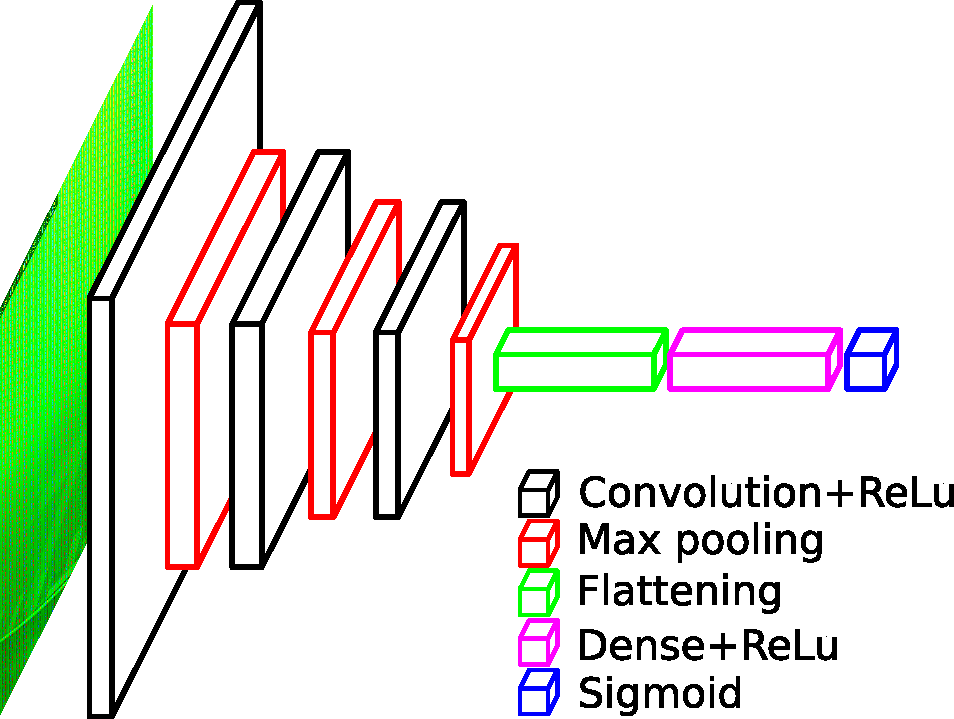
\includegraphics[width=\textwidth]{Figures/conv_net_fig}
    \caption{Architecture of the convolutional neural network.}
\end{figure}

\paragraph{The loss function:}
we are using in the \textit{ConvNet} is \textit{cross-entropy}.

\begin{equation}
    C(p,q) = -\sum_{i} p_i \log(q_i)
\end{equation}
$$\Longleftrightarrow$$
\begin{equation}
-y \log( \hat{y}) - (1-y)\log(1-\hat{y})
\end{equation}

\paragraph{Training:}
was done using a \textit{stochastic gradient descent} method known as the \textit{Adam-optimiser}.



%===  End of Marcus part
%======================================================================
\end{minipage}\hfill
\begin{minipage}[t]{0.30\textwidth}
%\vspace{-100pt}
%======================================================================
%===  Comparison part
\section*{Results}
\paragraph{Feature extraction approach:}
Table \ref{tab_rfc_2} reports the classification metrics from the Billund images. 

\begin{table}
\centering
\resizebox{\textwidth}{!}{
\begin{tabular}{ll|ll|llll}
 &  & \multicolumn{2}{l}{Pred.} & \multicolumn{4}{|l}{Class metrics} \\
 &  & Fog & Clear & Pre. & Sens. & F$_1$ & Acc. \\\hline
\multirow{2}{*}{\rotatebox[origin=c]{90}{Actual}} & Fog &  97 & 3 & 93 & 97 & 95 & 91 \\ 
 & Clear &80 & 20 & 35 & 20 & 26 & 91
\end{tabular}}
\caption{Performance metrics of predicting the appearance of fog in an unseen location. All values are in percentage.}
\label{tab_rfc_2}
\end{table}

The RFC does a poor job of detecting the appearance of clear weather in the unseen location. Therefore the generalization of the features is poor and location specific. 

\paragraph{Deep learning approach:}

\begin{table}
\centering
\resizebox{\textwidth}{!}{
\begin{tabular}{ll|ll|llll}
 &  & \multicolumn{2}{l}{Pred.} & \multicolumn{4}{|l}{Class metrics} \\
 &  & Fog & Clear & Pre. & Sens. & F$_1$ & Acc. \\\hline
\multirow{2}{*}{\rotatebox[origin=c]{90}{Actual}} 
 & Fog   & 87 & 13 & 91 & 87 & 89 & 89 \\ 
 & Clear & 9 & 91 & 88 & 91 & 89 & 89
\end{tabular}}
\caption{Performance metrics of predicting the appearance of fog. All values are in percentage.}
\label{tab_conv_1}
\end{table}

%Where do I begin?
%Answer these three questions:
%What is the most important / interesting / astounding finding from my research project?
%How can I visually share my research with conference attendees? Should I use charts, graphs, photos, images?
%What kind of information can I convey during my talk that will complement my poster?

\section*{Conclusion}
% Conclusion Anders
The handcrafted features are shown to be location specific and does not generalize to unseen locations. The RFC has an average accuracy of $98.5\%$ on the test set from Skive and an average accuracy of $58.5\%$ on unseen location from Billund.\\

The ConvNet proved to be quite effective, at an accuracy of $89.0\%$. It should be mentioned that given the sampling, Billund will very likely be over represented in the training, validation and test data sets.\\

So In all it seem to be the ANN which is performing best on the data but in order to be certain a bigger dataset and more tests are required.

%===  End of Comparison part
%======================================================================
\end{minipage}
%======================================================================
%===  Footnotes 
% This is the solution to the footnote problems. Add \footnotemark in the text and then set the texts here. Must be done in the same order.
\footnotetext[1]{The selected features are inspired by the presented features in "European Study Group with Industry 121" by M. Lyksborg et. al.}
%\footnotetext[2]{Copy kitting all over the place.}

%===  End of Footnotes 
%======================================================================
\end{document}
